\documentclass[12pt,a4paper,titlepage,headinclude,bibtotoc]{scrartcl}

%---- Allgemeine Layout Einstellungen ------------------------------------------

% Für Kopf und Fußzeilen, siehe auch KOMA-Skript Doku
\usepackage[komastyle]{scrpage2}
\pagestyle{plain}
\setheadsepline{0.5pt}[\color{black}]
\automark[section]{chapter}


%Einstellungen für Figuren- und Tabellenbeschriftungen
\setkomafont{captionlabel}{\sffamily\bfseries}
\setcapindent{0em}


%---- Weitere Pakete -----------------------------------------------------------
% Die Pakete sind alle in der TeX Live Distribution enthalten. Wichtige Adressen
% www.ctan.org, www.dante.de

% Sprachunterstützung
\usepackage[ngerman]{babel}

% Benutzung von Umlauten direkt im Text
% entweder "latin1" oder "utf8"
\usepackage[utf8]{inputenc}

% Pakete mit Mathesymbolen und zur Beseitigung von Schwächen der Mathe-Umgebung
\usepackage{latexsym,exscale,stmaryrd,amssymb,amsmath}


\usepackage[nointegrals]{wasysym}
\usepackage{eurosym}

% Anderes Literaturverzeichnisformat
%\usepackage[square,sort&compress]{natbib}
\usepackage{hyperref}
% Für Farbe
\usepackage{color}
\usepackage{graphicx}
\usepackage{wrapfig}
\usepackage{subfigure}

% Caption neben Abbildung
\usepackage{sidecap}


% Befehl für "Entspricht"-Zeichen
\newcommand{\corresponds}{\ensuremath{\mathrel{\widehat{=}}}}
% Befehl für Errorfunction
\newcommand{\erf}[1]{\text{ erf}\ensuremath{\left( #1 \right)}}


%Fußnoten zwingend auf diese Seite setzen
\interfootnotelinepenalty=1000

%Für chemische Formeln (von www.dante.de)
%% Anpassung an LaTeX(2e) von Bernd Raichle
\makeatletter
\DeclareRobustCommand{\chemical}[1]{%
  {\(\m@th
   \edef\resetfontdimens{\noexpand\)%
       \fontdimen16\textfont2=\the\fontdimen16\textfont2
       \fontdimen17\textfont2=\the\fontdimen17\textfont2\relax}%
   \fontdimen16\textfont2=2.7pt \fontdimen17\textfont2=2.7pt
   \mathrm{#1}%
   \resetfontdimens}}
\makeatother
\usepackage{textcomp}
\usepackage{upgreek}
%\begin{document}
%$\upmu$
%\end{document}
%Honecker-Kasten mit $$\shadowbox{$xxxx$}$$
\usepackage{fancybox}

%SI-Package
\usepackage{siunitx}

%keine Einrückung, wenn Latex doppelte Leerzeile
\parindent0pt

%Bibliography \bibliography{literatur} und \cite{gerthsen}
%\usepackage{cite}
\usepackage{babelbib}
\selectbiblanguage{ngerman}

\usepackage{siunitx}
%\begin{document}
 % \SI{1.55}{\micro\metre}
\sisetup{math-micro=\text{µ},text-micro=µ}
\begin{document}

\begin{titlepage}
\centering
\textsc{\Large Praktikum zur Einführung in die physikalische Chemie,\\[1.5ex] Universität Göttingen}

\vspace*{2cm}

\rule{\textwidth}{1pt}\\[0.5cm]
{\huge \bfseries
  V4: Molmassenbestimmung\\[1.5ex]
  durch Gefrierpunktserniedrigung}\\[0.5cm]
\rule{\textwidth}{1pt}

\vspace*{1cm}


\begin{Large}
\begin{tabular}{ll}
Durchführende: &  Alea Tokita, Julia Stachowiak\\
Assistentin: & Annemarie Kehl\\
 Versuchsdatum: & 07.12.2015\\
 Datum der ersten Abgabe: & 14.12.2015
\end{tabular}
\end{Large}

\vspace*{2cm}

\begin{Large}
\fbox{
  \begin{minipage}[t][5,5cm][t]{8cm} 
   Werte für Campher:\\
   $M_A = (13 \cdot 10 \pm 3 \cdot 10){~} \mathrm{g{~}mol^{-1}}$\\
   $M_B = (12 \cdot 10 \pm 2 \cdot 10){~} \mathrm{g{~}mol^{-1}}$\\\\
   Werte für Kaliumchlorid:\\
   $M_A = (6 \cdot 10 \pm 3 \cdot 10){~} \mathrm{g{~}mol^{-1}}$\\
   $M_B = (5\cdot 10 \pm 3\cdot 10 ){~} \mathrm{g{~}mol^{-1}}$\\
  
  \end{minipage}
}
\end{Large}

\end{titlepage}

\tableofcontents

\newpage

\section{Theoretische Grundlagen}

Bei idealen Lösungen stehen alle Moleküle in gleicher Wechselwirkung zueinander, egal ob sie vom Lösungsmittel oder der gelösten Komponente stammen. 
Wird nun eine Größe definiert, so können verschiedene Größen der Lösung mathematisch einfach getrennt werden. Ein Beispiel hierfür ist der Dampfdruck, welcher den isothermen Druck beschreibt, unterhalb dessen eine Flüssigkeit beginnt, in den gasförmigen Zustand überzugehen.
Der Dampfdruck\,$p$ einer Komponente $i$ in der Lösung setzt sich somit aus dem Dampfdruck der Komponente\,$p_{0i}$ und dem Stoffmengenanteil\,$x_i^l$ ebendieser in der Lösung bzw. flüssigen Phase\,$l$ zusammen.
Daraus ergibt sich das Raoult'sche Gesetz:\\

\begin{equation}
p_i = P_{0i} \cdot x_i^{l}
\end{equation}
\\

Da die Moleküle in realen Lösungen immer in Wechselwirkungen zueinander treten, ist die Abweichung vom Raoult'schen Gesetz sehr groß. Eine Näherung ergibt sich nur bei sehr geringen Wechselwirkungen und daher einer sehr geringen Molalität bzw. Konzentration des gelösten Stoffes: $x_i^2\,<<1$ und daraus für das Lösungsmittel $x_1^l\,= 1 - x_2^l$. Hier wird also davon ausgegangen, dass sich die Gasphase und flüssige Phase größtenteils aus dem Lösungsmittel zusammensetzen und der Dampfdruck der gelösten Substanz somit vernachlässigbar klein ist. Somit ergibt sich aus: \\

\begin{equation}
p_{ges} = p_1 + p_2 = p_{01} \cdot x_1^l + p_{02} \cdot x_2^l
\end{equation}

näherungsweise:
\begin{equation}
p_{ges} = p_{01} \cdot (1-x_2^l)
\end{equation}

Außderdem wird davon ausgegangen, dass sich beim Lösen des Stoffes keine Unregelmäßigkeiten wie z.B. Kristalle bilden, die den Idealitätscharakter der Lösung beeinflussen würden.\\

Dampf-, Schmelz-, und Sublimationsdruck der Lösung hängen somit nicht von der Art des gelösten Stoffes, sondern nur von der Temperatur und dem Lösungsmittel ab. So ergibt sich folgende Isochore (Abbildung 1):\\

\newpage

\begin{figure} [h!]
\begin{center}
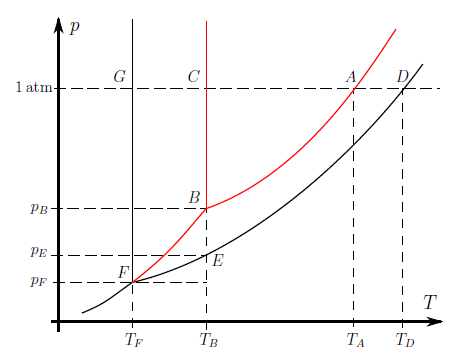
\includegraphics[scale=1]{Phasendiagramm.png} \end{center}
\caption {Zustandsdiagramm \protect\footnotemark}
\end{figure}
\footnotetext{Skriptum für das Praktikum zur Einführung in die Physikalische Chemie, Institut für physikalische Chemie, Uni Göttingen, 2015, Seite 24}

Die rote Linie zeichnet die Übergänge der Aggregatzustände des reinen Lösungsmittels. Nahe der Abszisse (dh. bei geringer Temperatur) ist der feste Bereich und nahe der Ordinate (bei geringem Druck) der gasförmige.
Somit bildet die Strecke $\overline{AB}$\,mit dem Übergang zwischen gasförmigen und flüssigem Zustand den Dampfdruck; $\overline{BC}$\,den Schmelzdruck. $\overline{FB}$\,beschreibt den Sublimationsdruck und $C$\, den Gefrierpunkt (bei\,$p= 1\,\mathrm{atm}$).\\
Die schwarze Kurve zeigt die Phasenübergänge der Lösung; die Bezeichnungen für die jeweiligen Streckenabschnitte gelten hier analog.\\
Auffällig ist die Verschiebung des Tripelpunktes, die nah mit der Differenz der Gefrierpunkte, dh. der Gefrierpunktserniedrigung\,$\Delta T_g = T_C - T_G$ zusammenhängt. \\
Der fast senkrechte Anstieg der Gefrierpunktserniedrigung\,$T_g$ entspricht somit näherungsweise der Verschiebung des Tripelpunktes und es ergibt sich:  \\

\begin{equation}
T_G \approx T_B - T_F
\end{equation}

\newpage

Diese kann mithilfe der Steigung der Dampfdruck- und Sublimationsdruckkurven errechnet werden. Das Raoultsche Gesetz besagt:\\

\begin{equation}
p_B - p_E = p_B \cdot x_2^l
\end{equation}
\\

Für die Steigung der Dampfdruckkurve und Sublimationsdruckkurve wird ebenfalls ein linearer Verlauf angenommen. Wie auf Abbildung 1 ersichtlich besitzen sie näherungsweise dieselbe Steigung, sodass gilt:\\

\begin{equation}
\dfrac{p_B - p_E}{\Delta T_g} = \frac{\Delta p}{\Delta T}\bigg \vert_{Subl} - \frac{\Delta p}{\Delta T}\bigg \vert_{Dampf}
\end{equation}

Einsetzen der Druckdifferenz $p_B - p_E$ aus dem Raoultschen Gesetz ergibt nach Umformung für\,$T_g$:\\

\begin{equation}
\Delta T_g =\dfrac{p_B \cdot x_2^l}{\frac{\Delta p}{\Delta T}\bigg \vert_{Subl} - \frac{\Delta p}{\Delta T}\bigg \vert_{Dampf}}
\end{equation}
\\

Der Stoffmengenanteil\,$x_2^l$ ist proportional zur Molalität\,$\check c$ . Der Rest der Gleichung ist stoffabhängig und kann mit der stoffspezifischen kryoskopischen Konstante\,$\Theta_g$ zusammengefasst werden, welche die Schmelz- bzw. Gefierpunktsänderung darstellt:

\begin{equation}
\Delta T_g = \Theta_\mathrm{g} \cdot \check c = \Theta_\mathrm{g} \cdot \frac{m_\mathrm{2}}{M_\mathrm{2} \cdot m_\mathrm{1}}
\end{equation}

Somit ist die Erniedrigung bzw. Erhöhung des Gefrierpunktes eine kolligative Eigenschaft; die Veränderung ist nur von der Menge des gelösten Mittels, nicht aber ihrer Konsistenz abhängig. Die Gleichung trifft nur zu, solange keine Mischkristalle ausfallen.\\

%Analog für die Siedepunktserhöhung ergibt sich die ebullioskopische Konstante\,$\Theta_S$:\\

%\begin{equation}
%\Delta T_\mathrm{S} = \Theta_\mathrm{S} \cdot \check c = \Theta_\mathrm{S} \cdot \frac{m_\mathrm{2}}{M_\mathrm{2} \cdot m_\mathrm{1}}
%\end{equation}

Die hier angegebene Molmasse ist nicht komplett äquvalent zu der tatsächlichen Molmasse der gelösten Substanz, da sie nicht komplett dissoziiert. Somit ergibt sich unter Anbetracht des Dissoziationsgrades $\alpha$ für die tatsächliche Molmasse: \\

\begin{equation}
M_2 = \frac{M_\mathrm{02}}{1+(z-1) \cdot \alpha}
\end{equation}

\section{Experimentelles}
\subsection{Prinzip des Experiments}

Ziel des Versuches ist es, die Molare Masse einer Substanz mithilfe ihrer Gefrierpunktserniedrigung im Bezug auf ein Lösungsmittel aus letzterer Gleichung zu bestimmen. Als Lösungsmittel sind Cyclohexan und Wasser gegeben, jedem Lösungsmittel zugehörig eine unbekannte Substanz.\\
Es können sich folgende Abkühlungskurven bilden, anhand derer der Gefrierpunkt extrapoliert werden soll (gestrichelte Linie): 

\begin{figure} [h!]
\begin{center}
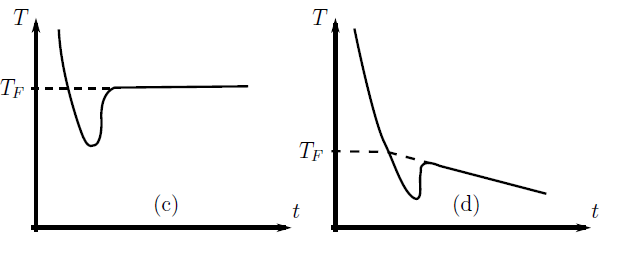
\includegraphics[scale=0.8]{Abkuhlungskurven.png} \end{center}
\caption {Abkühlungskurven. \protect\footnotemark}
\end{figure}
\footnotetext{Skriptum für das Praktikum zur Einführung in die Physikalische Chemie, Institut für physikalische Chemie, Uni Göttingen, 2015, Seite 28}

Der vorübergehende schnelle Abfall unter den Gefrierpunkt, Unterkühlung, ist darauf zurückzuführen, dass bei Gefrieren der Lösung vorerst ein inhomogenes System aus einem homogenen System entsteht. Für diesen energieaufwändigen Prozess der Keimbildung wird dem System Energie in Form von Wärme entzogen, welches sich in der Unterkühlung beobachten lässt.


\subsection{Versuchsaufbau}



\begin{figure} [h!]
\begin{center}
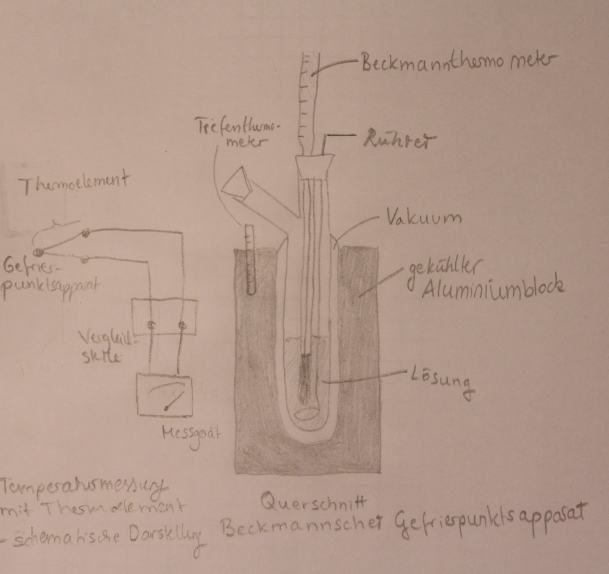
\includegraphics[scale=0.8]{Versuchsaufbau2.png} \end{center}
\caption{Versuchsaufbau.}
\end{figure}

\subsection{Durchführung}

Der Versuch wird in zwei Gruppen aufgeteilt ausgeführt, wobei eine Gruppe die Gefrierpunktserniedrigung eines Lösungsmittels misst. \\
Zuerst wird der Versuch wie auf der Skizze ersichtlich aufgebaut und das Beckmannthermometer auf einen Temperaturbereich geeicht.
 Die Vergleichsstelle des Thermoelements wird in ein Wasser-Eisbad getunkt und das Element an elektronisches Speichermedium angeschlossen.\\
 
 Zuerst wird der Aluminiumblock mit flüssigem Stickstoff auf ca. $-30 ^\circ\text{C}$ bei Wasser als Lösungsmittel und ca. $-15 ^\circ\text{C}$ bei Cyclohexan gekühlt. Anschließend werden 20 mL des Lösungsmittels in das innere Reagenzglas einpipettiert und dieses in den Aluminiumblock gestellt. Nun wird unter Rühren alle 10 Sekunden die Temperaturänderung erfasst, bis keine oder nur noch eine sehr schwache Temperaturänderung wahrnehmbar und die Lösun fest geworden ist. \\
 Nach Auftauen des Lösungsmittels und erneutem Kühlen des Aluminiumblockes auf die entsprechende Temperatur werden 0,32\, g bei Wasser und 0,16\,g bei Cyclohexan der Substanz mit unbekannter Molmasse hinzugefügt und die Messung der Temperaturänderung wiederholt und in gleichen Intervallen notiert.\\
Nach Wiederauftauen wird erneut die möglichst gleiche Menge Versuchssubstanz abgewogen und beigefügt. Der Vorgang wird wie oben beschrieben wiederholt und die Ergebnisse notiert. Als Messergebnisse ergeben sich drei Gefrierpunktskurven, aus denen der Gefrierpunkt grafisch extrapoliert werden kann.\\
 
 
 







\section{Auswertung}

\subsection{Messergebnisse für Cyclohexan}

Volumen des Lösungsmittels: $V_{\mathrm{Cyclohexan}} = 0,02 {~} \mathrm{L}{~}\widehat{=}{~}20 {~}\mathrm{cm^3}$ \\
Masse des Lösungsmittels:  $m_{\mathrm{Cyclohexan}} = {~} \rho \cdot V = 0,78{~} \mathrm{g {~}cm^{-3}} \cdot 20{~} \mathrm{cm^{3}} = 16{~}\mathrm{g}$\\
Masse der Einwaage A: $m_A = 0,1613{~} \mathrm{g}$\\ 
Masse der Einwaage B: $m_B = 0,1655{~} \mathrm{g}$\\
$\Theta _g = 20,2 {~} \mathrm{kg{~}K {~} mol^{-1}}$\\\\
Gefrierpunkt des reinen Lösungsmittel: $ T_g = 6,4 {~}^{\circ}\text{C}$\\
Gefrierpunkt der Lösung A: $ T_{gA} = 4,8 {~}^{\circ}\text{C}$\\
Gefrierpunkt der Lösung B: $ T_{gB} = 2,9 {~}^{\circ}\text{C}$\\
$ \Delta T _{gA} = T_g - T _{gA} = 6,4 {~}^{\circ}\text{C} - 4,8 {~}^{\circ}\text{C} = 1,6 {~}^{\circ}\text{C} = 1,6{~}\mathrm{K} $\\
$ \Delta T _{gB} = 6,4 {~}^{\circ}\text{C} - 2,9 {~}^{\circ}\text{C} = 3,5 {~}^{\circ}\text{C} = 3,5 {~} \mathrm{K} $
\subsection{Messergebnisse für Wasser}

Volumen des Lösungsmittels: $V_{\mathrm{Cyclohexan}} = 0,02 {~} \mathrm{L}{~}\widehat{=}{~}20 {~}\mathrm{cm^3}$ \\
Masse des Lösungsmittels:  $m_{\mathrm{Cyclohexan}} = {~} \rho \cdot V = 1,00{~} \mathrm{g {~}cm^{-3}} \cdot 20{~} \mathrm{cm^{3}} = 20{~}\mathrm{g}$\\
Masse der Einwaage A: $m_A = 0,316{~} \mathrm{g}$\\ 
Masse der Einwaage B: $m_B = 0,316{~} \mathrm{g}$\\
$\Theta _g = 1,86 {~}\mathrm{kg{~}K {~} mol^{-1}}$\\\\
Gefrierpunkt des reinen Lösungsmittel: $ T_g = -1,4 {~}^{\circ}\text{C}$\\
Gefrierpunkt der Lösung A: $ T_{gA} = -2,5 {~}^{\circ}\text{C}$\\
Gefrierpunkt der Lösung B: $ T_{gB} = -3,5 {~}^{\circ}\text{C}$\\
$ \Delta T _{gA} =  1,1 {~}^{\circ}\text{C} = 1,1 {~}\mathrm{K} $\\
$ \Delta T _{gB} = 2,1 {~}^{\circ}\text{C} = 2,1{~} \mathrm{K} $

\subsection{Bestimmung der Molmasse:}

Es gilt folgender Zusammenhang:
\begin{equation}
\Delta T_g = \Theta _g \cdot \frac{m_2}{M_2 \cdot m_1}
\end{equation}

Daraus lässt sich folgende Formel zum Ermitteln der Molmasse aufstellen:
\begin{equation}
 M = \frac{\Theta _g \cdot m_2 }{ \Delta T_g\cdot m_1}
\end{equation}

\subsection{ Bestimmung der Molmasse der Substanz in Cyclohexan}

Durch Einsetzen der Messergebnisse in die obige Gleichung ergibt sich für Lösung A:\\

$M_A = \frac {\Theta _g \cdot m_2 }{ \Delta T_g\cdot m_1} 
 = \frac {20,2{~} \mathrm{kg{~}K {~} mol^{-1}} \cdot 0,1613 {~}\text{g}} { 1,6 {~} \mathrm{K} \cdot 15,6{~} \mathrm{g}} \approx 0,13{~} \mathrm{kg {~} mol^{-1}} {~}\widehat{=}{~} 13 \cdot 10{~} \mathrm{g{~}mol^{-1}} $\\

Und für Lösung B:\\

$M_B \approx 12 \cdot 10{~} \mathrm{g{~}mol^{-1}}$


\subsection{Bestimmung der Molmasse der Substanz in Wasser}

Die Molmasse berechnet sich analog zu der obigen Rechnung. Es ergibt sich für Lösung A:\\
$M_A^{'} \approx 27{~} \mathrm{g{~}mol^{-1}}$\\\\
Und für Lösung B:\\
$M_B^{'} \approx 28{~} \mathrm{g{~}mol^{-1}}$\\\\

Diese ist jedoch nur eine scheinbare Molmasse. Da die Substanz im Wasser in Ionen dissoziiert, in diesem Fall in eine Anion und ein Kation (es handelt sich um KCl) muss das Ergebnis noch mit dem Faktor zwei multipliziert werden. Somit ergibt sich:\\\\
$M_A = M_A^{'} \cdot 2 \approx 56{~} \mathrm{g{~}mol^{-1}} $\\
$M_B = M_B^{'} \cdot 2 \approx 53{~} \mathrm{g{~}mol^{-1}} $\\

\section{Fehlerrechnung}
\subsection{Fehlerfortpflanzung}
Folgende Gerätefehler werden abgeschätzt:\\

$\Delta m_1 = 1{~}\mathrm{g}  $\\
$\Delta m_2 = 0,001{~}\mathrm{g}  $\\
$\Delta (\Delta T_g) = 0,5{~}\text{K}  $\\ Dies ist der abgeschätzte Fehler für das Beckmann Thermometer.\\\\
Da jedoch mit den Messungen aus der Auftragung gerechnet wird muss der Fehler für die elektronische Messung graphisch aus der Auftragung bestimmt werden. Dabei werden aus den Schwankungen der Graphen maximale und minimale Gefrierpunkte ermittelt, wodurch sich ebenfalls maximale und minimale Gefrierpunktdifferenzen bestimmen lassen. Nun lässt sich der absolute Fehler für $\Delta (\Delta T_g)$ mithilfe folgender Formel bestimmen:
\begin{align}
\Delta (\Delta T_g) = \dfrac{ \Delta T_{g\mathrm{~}{max}}-\Delta T_{g\mathrm{~}{min}}}{2}
\end{align}

Somit ergibt sich für die Messung mit Wasser als größter möglicher Fehler $\Delta (\Delta T_g) = 0,2{~\mathrm{K}}$  und für Cyclohexan $\Delta (\Delta T_g) = 0,3{~\mathrm{K}}$

Der Fehler $\Delta M$ lässt sich durch die Gaußsche Fehlerfortpflanzung berechnen, dadurch erhält man folgende Formel:

\begin{align}
\Delta M = \sqrt{ \left( \frac {\Theta _g}{ \Delta T_g\cdot m_1} \cdot \Delta m_2 \right)^2 + \left( \frac {\Theta _g \cdot m_2 }{ \Delta T_g\cdot m_1^2 } \cdot \Delta m_1 \right)^2 + \left( \frac {\Theta _g \cdot m_2 }{ \Delta T_g^2 \cdot m_1} \cdot \Delta (\Delta T_g) \right)^2 } \cdot 1000
\end{align}

Hierbei wird $\mathrm{mit {~}1000}$ multipliziert, sodass überall mit der Einheit $\mathrm{g}$ gerechnet wird und der Fehler sich auf das Ergebnis $\mathrm{g{~} mol^{-1}}$ bezieht.

Somit ergeben sich für die Fehler der Molmasse der Substanz in Cyclohexan:\\


$\Delta M_\mathrm{A} = \sqrt{ \left( \frac {20,2 {~}\mathrm{kg {~} K {~} mol^{-1}}}{ 1,6 {~} \mathrm{K} \cdot 16 {~}\mathrm{g}} \cdot 0,001 \mathrm{g} \right)^2 + \left( \frac { 20,2 {~}\mathrm{kg{~}K {~} mol^{-1}} \cdot 0,1613{~}\mathrm{g} }{ 1,6 {~}\text{K}\cdot (16 {~}\mathrm{g} )^2 } \cdot 1 {~} \mathrm{g} \right)^2 +  \left( \frac {20,2 {~}\mathrm{kg{~}K {~} mol^{-1}} \cdot 0,1613 {~} \mathrm{g}} { 16 {~} \mathrm{g} \cdot (1,6 {~} \text{K})^2} \cdot 0,3{~} \text{K} \right)^2}  $
\begin{align}
\cdot 1000 = 3 \cdot 10{~}\mathrm{g{~}mol^{-1}}
\end{align}


$\Delta M_\mathrm{B} = 2 \cdot 10 {~}\mathrm{g{~}mol^{-1}}$\\\\

Weiterhin ergibt sich für die Fehler in den Molmassen der Substanz im Wasser:\\
$\Delta M_\mathrm{A} = 3 \cdot 10  {~}\mathrm{g{~}mol^{-1}} $\\
$\Delta M_\mathrm{B} = 3 \cdot 10 {~}\mathrm{g{~}mol^{-1}}$\\

\subsection{Diskussion Systematischer Fehler}
Zu den abgeschätzten Gerätefehlern kommen noch weitere systematische Fehler, welche das Ergebnis beeinflussen. Zunächst wird mit einigen Näherungen gerechnet, welche zu Abweichungen im Ergebnis führen können.\\\\
Des weiteren gibt es einige Ungenauigkeiten im Messen der Temperatur der Lösung. Die nach Augenmaß abgelesenen Werte sind sehr ungenau, es ist schwierig, exakt alle zehn Sekunden richtig abzulesen. Hierbei kommt es vor allem zu Verspätungen aufgrund der menschlichen Reaktionszeit.\\\\ Daher ist die elektronische Messung zu bevorzugen, welche jedoch auch Fehler enthalten kann. Etwa ist die Eichflüssigkeit, Eiswasser, mit der Zeit immer wärmer geworden, ebenfalls ist das Thermoelement leicht zu beeinflussen, beispielsweise durch den versehentlichen Kontakt zum Rührstab. Letztere Beeinflussung lässt sich meist gut graphisch ausgleichen. Das Erwärmen des Eiswassers könnte jedoch zur Folge haben, dass die Temperaturen der Lösungen immer zu hoch oder zu niedrig gemessen werden. So könnte sich bei einer sich daraus ergebenden beispielsweise zu kleinen Temperaturdifferenz, eine zu große Molmasse ergeben.\\\\
Weiter Fehler entstehen auch im Abwiegen der Massen $M_1$ und $M_2$. Vor allem $M_2$ wird lediglich pipetiert, sodass es dadurch zu Fehlern kommt. Wird $M_2$ dabei etwa zu groß gemessen, hätte dies auch eine zu große Molmasse zur Folge. Des weiteren gibt es Ungenauigkeiten bei der Masse $M_2$, oft sind Reste der Substanz im Schippchen, zum Abwiegen, hängen geblieben, was bei den sehr kleinen abgewogen Mengen zu Fehlern führt. Die zweite Substanz, Campher, ist hygroskopisch, auch die führt zu Ungenauigkeiten im Abwiegen.\\\\
Zur Bestimmung des Gefrierpunktes muss wegen der Unterkühlung extrapoliert werden, dies ist allerdings nur mit sehr kleinen Fehlern behaftet.

\section{Diskussion}
\subsection{Vergleich mit den Literaturwerten}
Für die Molmasse der Substanz im Cyclohexan ergeben sich folgende Werte:\\\\
$M_A = (13 \cdot 10 \pm 3 \cdot 10){~} \mathrm{g{~}mol^{-1}}$\\\\
$M_B = (12 \cdot 10 \pm 2 \cdot 10){~} \mathrm{g{~}mol^{-1}}$\\\\
Dabei handelt es sich um Campher, dieses hat eine Molmasse von $ 152,23{~} \mathrm{g{~}mol^{-1}}$ \footnote{https://de.wikipedia.org/wiki/Campher abgerufen am \textbf{13.12.2015}} Der erste Wert liegt mit den Fehlerintervallen ein wenig unterhalb dieses Wertes, der zweite Wert weicht zu weit nach unten ab. Beide Werte weichen nach unten hin ab, dies legt einen systematischen Fehler nahe.\\\\
Für die Molmasse der im Wasser gelösten Substanz ergibt sich:\\\\
$M_A = (6 \cdot 10 \pm 3 \cdot 10){~} \mathrm{g{~}mol^{-1}}$\\\\
$M_B = (5\cdot 10 \pm 3\cdot 10 ){~} \mathrm{g{~}mol^{-1}}$\\\\
Es handelt sich bei der im Wasser gelösten Substanz um Kaliumchlorid, dieses hat eine Molmasse von $74,55{~} \mathrm{g{~}mol^{-1}}$ {~}\footnote{https://de.wikipedia.org/wiki/Kaliumchlorid abgerufen am \textbf{09.12.2015}} Diese Molmasse liegt in den Fehlerintervallen beider Werte. Auch hier gibt es eine Abweichung nach unten, was denselben systematischen Fehler wie bei der Messung mit Cyclohexan nahe legt. 


\subsection{Disskussion} 
Der Wert liegt auch mit dem Fehler nicht in dem Bereich der tatsächlichen Molmasse. Dies lässt sich durch bereits diskutierte systematische Fehler erklären. Des weiteren ist die Berechnung nicht ganz exakt, an einigen Stellen wurde mit vereinfachten Näherungen gerechnet. Etwa wird von der Gültigkeit des Raoult´schen Gesetz ausgegangen, wobei dies vor allem für sehr geringe Konzentrationen an Lösungsmittel gilt. Auch sind die Gleichungen zunächst auf den Stoffmengenanteil $x_2^l$ bezogen, der dann näherungsweise in $c_2^l$ umgerechnet wird. Dabei wird davon ausgegangen, dass bei hoher Konzentration des Lösungsmittels gilt:
\begin{align}
x_2^l = \dfrac{n_B}{n_A + n_B} = \dfrac{n_B}{n_A}
\end{align}   

So wird durch weiteres Einsetzen die Molalität der gelösten Substanz $c_2^l$ multipliziert mit der Molmasse des Lösungsmittels erhalten, welche in die Kryoskopische Konstante gezogen wird. Besonders diese Näherung ist je nach Menge an gelöster Substanz eine sehr grob. Im Versuch wurden bis zu $0,7{~}\mathrm{g}$ Substanz verwendet, welches immerhin eine Stoffmenge von fast $n_B = 0,01${~}mol ergibt. Setzt man diese größtmöglichen Werte für die Stoffmengen in die obige Gleichung ein ergibt sich eine Abweichung von lediglich $1 {~} \% $, man kann also von einer guten Näherung sprechen. Für genauere Ergebnisse sollte dies Berechnung jedoch exakt durchgeführt werden. Des weiteren wäre es sinnvoll ein Mittelwert aus den erhaltenen Molmassen zu bilden.  
 


 














\newpage



\subsection{Literaturverzeichnis}
1\quad Götz, Eckhold: \emph{Sriptum zur Einführung in die physikalische Chemie}, Institut für physikalische Chemie, Uni Göttingen, \textbf{2015}.

\vspace{0,5 cm}

2 \quad https://de.wikipedia.org/wiki/Campher abgerufen am \textbf{13.12.2015}

\vspace{0,5cm}

3 \quad https://de.wikipedia.org/wiki/Kaliumchlorid abgerufen am \textbf{09.12.2015}

\vspace{0,5cm}

4 \quad \emph{Skriptum für das Praktikum zur Einführung in die Physikalische Chemie}, Institut für physikalische Chemie, Uni Göttingen, \textbf{2015}.\\










\end{document}


